% BASED ON SIGPROC-SP.TEX - VERSION 3.1

%\documentclass[final,reprint,notitlepage,narroweqnarray,inline,twoside,invited]{ieee}

\documentclass{acm_proc_article-sp}
\usepackage{graphicx}

\begin{document}

\title{{\ttlit ModelDoc}: Auto-generated, Auto-regenerated Wiki-Based Database Documentation}

\numberofauthors{2}
\author{
  \alignauthor
  Jim Steinberger\\
         \affaddr{College of Engineering}\\
         \affaddr{University of Michigan}\\
         \affaddr{Ann Arbor, MI, USA}\\
         \email{jsteinbe@eecs.umich.edu}
  \alignauthor
  Atul Prakash\\
         \affaddr{College of Engineering}\\
         \affaddr{University of Michigan}\\
         \affaddr{Ann Arbor, MI, USA}\\
         \email{aprakash@eecs.umich.edu}
}

\maketitle

\begin{abstract}
Software developers often find databases difficult to work with because they
are not documented properly.  When documentation does exist, it is often
inaccurate, out-of-date, and/or unclear.  In this paper, we present ModelDoc --
an extension on MediaWiki -- as a new approach to documenting databases and,
potentially, other aspects of an application.  ModelDoc will auto-generate
documentation from a live data source, and it then continually auto-regenerates
that documentation as the data source changes.  The documentation is consistent
and kept up-to-date, but also exists along the standard wiki functionality,
allowing collaboration throughout the evolution of the database.
\end{abstract}

\category{H.4}{Information Systems Applications}{Miscellaneous}
\category{D.2.7}{Software Engineering}
{Distribution, Maintenance, and Enhancement}

\terms{wiki, database, database schema evolution, documentation, auto-generated
documentation}

\section{Introduction}
The problem of software documentation is well-known but rarely explored. 
Documentation is often missing, or when it does exist, it is out-of-date,
incomplete, and/or simply inaccurate.  There are countless reasons for
this lack of documentation -- an absence of technical writers on a team, a
perception that documentation is optional and only to be done during ``free
time,'' the intractability of documenting a large legacy system, etc. -- but
they can usually be summed up as: documentation is not easy to write and
maintain.  Even when documentation is created initially, as the project changes
the documentation falls out of date, making it harder to change the project
further, often leading to project stagnation or failure
\cite{desouza:documentation} \cite{sousa:maintenance}.

Collaborative documentation is also increasingly important. 
Contemporary software projects are almost never individual endeavors. Projects
often have large teams of developers working on them, and these developers have
different perspectives and sets of knowledge.  Further, teams are increasingly
inter-disciplinary.  The project that inspired ModelDoc was made up of not only
developers, but also mechanical, electrical, and structural engineers -- the project cannot be properly understood without specialized descriptions from all these players.

The challenge of maintaining documentation throughout the evolution of a
project compounds these challenges.  Software is constantly updated and
changed, and the documentation needs to be updated to reflect these changes.
 Outdated documentation is often worse than a lack of documentation, as bad
assumptions about the behavior of code can result in more wasted time than
when a developer is forced to derive code's behavior from the code itself.

Databases are particularly difficult to document well.  While it is generally
easy to generate documentation from source code, there is little analogous
tool-support for databases.  The tools that do exist require human attention to
manage and maintain, and the generated documentation is not easily collaborated
over and consequently lacks perspective. The hampered utility of these
documents, coupled with the challenges of a small group of people trying to
manually keep this documentation updated -- often leads to
documentation-stagnation.

Here we present ModelDoc, a MediaWiki (\cite{web:mediawiki}) extension that
provides a wiki-based approach to documenting database schemas.  The benefits of collaborative
documentation via a wiki are well-known, but a development team cannot simply install a wiki
and expect documentation to suddenly become easy to maintain.  ModelDoc is an
attempt to address many of the obstacles between development teams and quality
documentation by integrating the classic benefits of creating documentation
with a wiki (easy collaboration, versioning, etc.) with auto-generated and
auto-synched content.

At the time of this writing, ModelDoc queries metadata from a live database to
generate structured wiki pages from that metadata.  This design choice is
partly due to ease-of-implementation, but it should be noted that today's
gigantic, web-accessible databases are expected to be online 24/7, and there
are many attempts to reorganize databases while keeping them online
\cite{sockut:reorganization} \cite{curino:evolution}.  Regardless, ModelDoc can
readily be extended to use SQL files, ORM mapping-files, XML files, and perhaps
even source code.

\section{Goals / Contributions}

ModelDoc seeks to achieve mutual consistency between a database and its
documentation.  When someone makes a change to a project's database, the
corresponding documentation should be updated in a useful way.  Further, people
interested in that documentation should be notified of the update so they may
investigate/affirm it.  The author of a bit of documentation should be
identifiable, and the version-history for documentation should be explorable. 
Generated data should be clearly presented, and relationships to other
data/entities should be clear.

Some of these goals -- e.g. versioning, authorship -- are accomplished by the
underlying wiki.  ModelDoc's contribution is its bridging of the benefits
wikis have provided static documentation to the dynamic needs of software
projects.

An important side-goal has been to provide a platform for future extensions. 
As implied by the Future Work section, there are multiple promising ways in
which this approach could be extended to address other documentation challenges
in software development.

\section{Related Work}
As far as we know, this is the first attempt to utilize a wiki to document a
database system.

Industry tools for database documentation have generally taken the approach of
having users manually creating and laying out an ER diagram; such is
the approach of tools like Microsoft Visio and Omnigroup's Omnigraffle.  There

is some industry support for the auto-generation and regeneration of database

documentation: Visio has some support for keeping an ER diagram in synch with a

database's metadata, and SchemaSpy will generate a series of graphical and

textual documents based on this metadata. However, these auto-generated

diagrams rarely capture the right visual organization that makes such diagrams

useful.



There are also tools for auto-generating documentation for non-database work,

such as the *Doc family of tools for documenting source code (JavaDoc, PHPDoc,

JSDoc, Doxygen, etc).  These tools generally, however, produce read-only

documentation.  JavaDoc, for example, generates HTML files; once generated

there can be little collaboration and discussion on whether the business domain

has been successfully modeled.



There has been work at creating algorithms for summarizing complex schemas

\cite{jag:summarization} \cite{yang:summarizing}, but as with the *Doc tools,

this is a read-only view of the schema.  These approaches are helpful for

querying complex systems, but they assume their users correctly understand

what the fields and entities truly \textit{mean}; there still needs to be

collaborative documentation and agreement on the semantics of a system, and

how/why they have evolved over time.



Algorithms have also been explored for ``redocumentation''

\cite{rajlich:webredoc}, creating new/different documentation for/from a

system, as well as attempts to automate this process \cite{anquetil:atool}.



Temporal informatics, the study of how information changes over time (e.g. on

the web \cite{adar:zoetrope}), is certainly relevant, but has not yet been

applied specifically to software documentation, and the obstacles and issues

surrounding documentation's evolution over time.



\section{ModelDoc}



ModelDoc extends MediaWiki's existing functionality through MediaWiki's

standard extension framework.  ModelDoc currently works with Postgres

databases, but features an extension API for interfacing with other

entity-relational data sources, and potentially non-relational database data

sources as well.



\subsection{Overview}



ModelDoc is MediaWiki extension, built using PHP5 and deployed into an existing

MediaWiki installation using the standard procedure.  Unlike wikis that

encourage more open collaboration, though, a ModelDoc-enabled wiki for a

proprietary project will likely involve stronger security considerations.



Database metadata is obtained via live database connections.  A single ModelDoc

installation can work with an arbitrary number of databases -- the

configuration for these connections is stored in a special ModelDoc wiki page

(see Special Pages).



Members of a project use the wiki in the standard way, collaborating through

the creation and updating of wiki pages.  All the standard wiki-functionality

is maintained and encouraged: version-history for pages, using the

``discussion'' pages for meta-documentation of a page, ``watching'' pages to be

notified when they are updated, etc.



ModelDoc extends MediaWiki, however, with special tags that users can use when

creating documentation.  For example, by adding an ``entity-list'' tag to a

page, and specifying a data source (see Tags section), when later viewing that

page, ModelDoc will query the data source and generate a list of the tables in

that database.  Further, each entry in this list will be a link to a

ModelDoc-generated page containing the table's metadata (columns,

constraints, etc.) and documentation.



For each of these entity-pages, ModelDoc also creates a corresponding HISTORY

page containing -- in XML format -- the last-seen set of metadata for the

table.  This metadata is compared to the live data every time the tag generates

content; ModelDoc compares this information to see what has been added and what

is missing, and appends these changes to the respective pages.  Thus, when

viewing an entity-page, the user sees not only the current information for the

database table, but also an auto-generated history of how that table has

evolved over time.  These sections are editable, the project members can (and

are encouraged to -- see the Special Pages section for ``ModelDoc::To Document''

) update/replace these sections with documentation that is more comprehensive

and user-friendly.



\begin{figure}[b]

\centering

%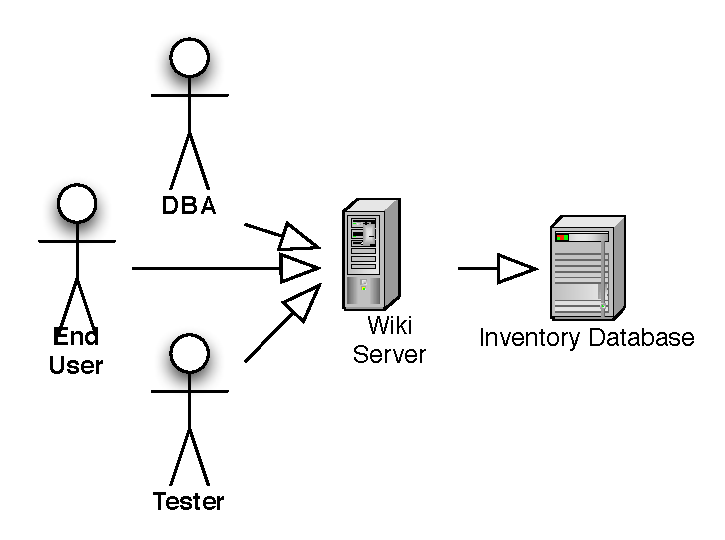
\epsfig{file=Overview.pdf}

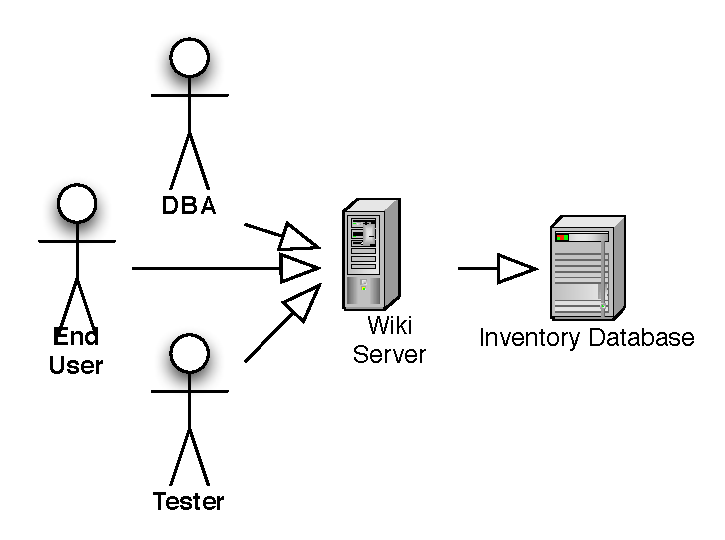
\includegraphics[width=220px]{Overview.pdf}

\caption{Overview of a sample ModelDoc system.}

\end{figure}



\begin{figure}

\centering

%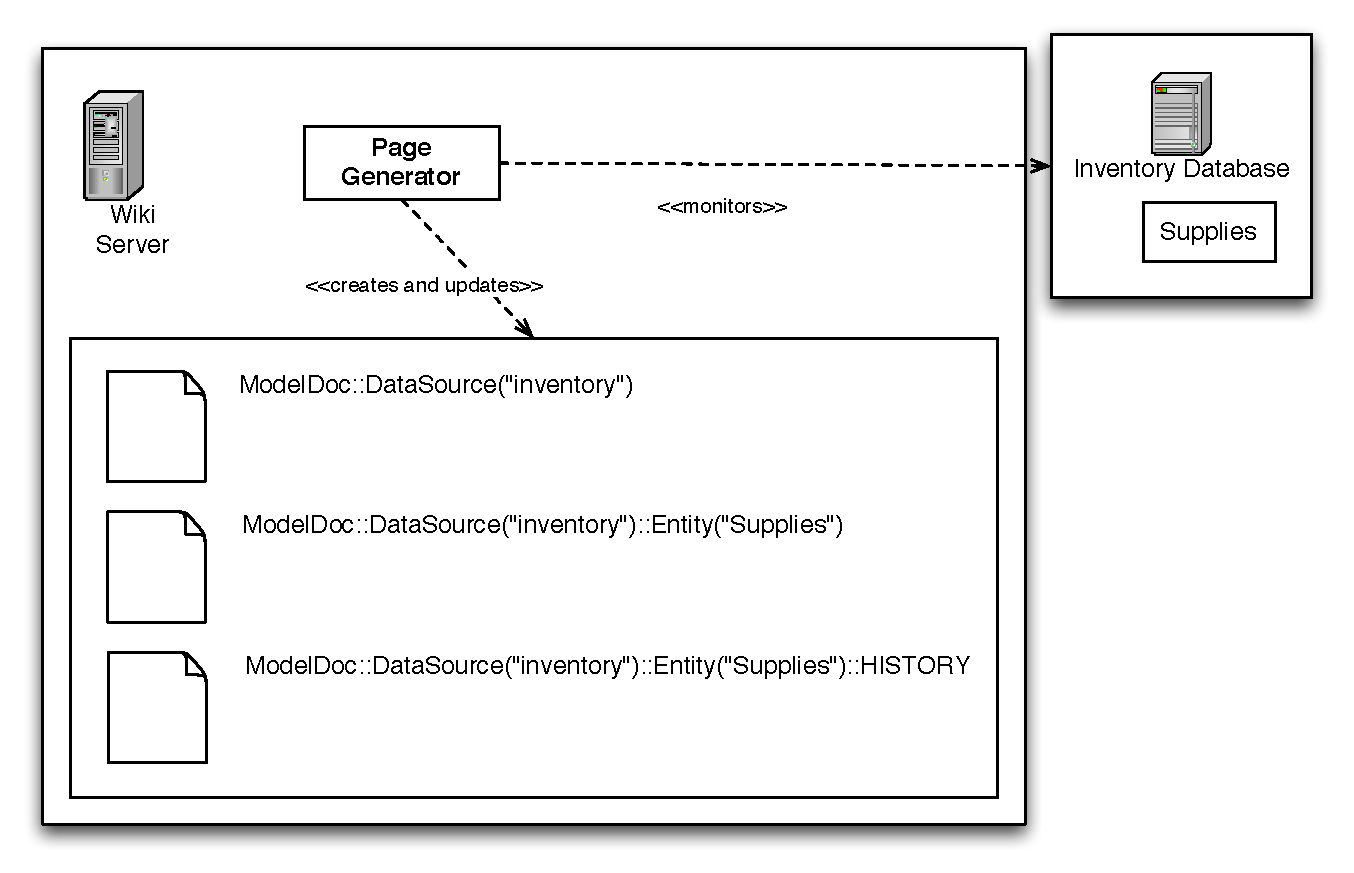
\epsfig{file=PageManager.pdf}

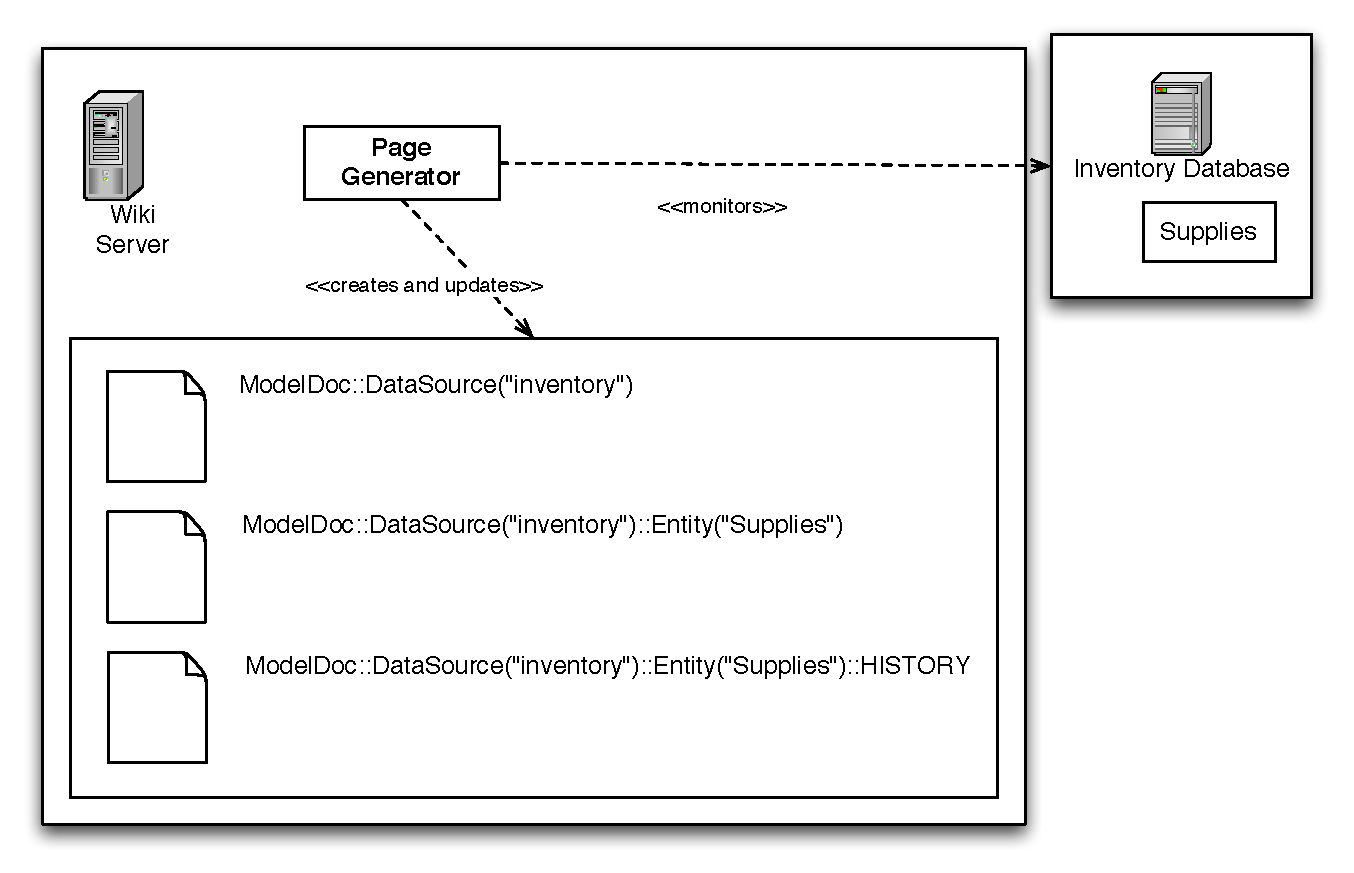
\includegraphics[width=250px]{PageManager.pdf}

\caption{The role of ModelDoc's page-manager component.}

\end{figure}



\subsection{Data Sources}



In ModelDoc, a data source represents a resource that contributes information

about the model of an application -- currently Postgres and MySQL databases, but

potentially data sources ranging from other relational databases to XML files

to annotated source code to other wiki pages.  ModelDoc queries metadata from

data sources for information about the entities, and then monitors the data

sources for changes to those entities.



Each data source may contribute its own set of entities.  Currently, data

sources are considered independent of each other, and it is further assumed

that a database table represents a single database entity.  A possible

extension is to follow the example of object-relational mappers and provide

a way to map an entity to multiple database tables, or a database table to

multiple entities.



For example, consider a ``Person'' entity.  In a

properly-normalized database, chances are that the information that constitutes a ``Person'' will be spread

out over multiple tables, such as an ``Address'' table.  ModelDoc currently

requires that these be considered separate entities in the documentation.



\subsection{Versioning}



For each entity, ModelDoc automatically generates a companion read-only page

that maintains the entity's history.  This companion page maintains XML-based

metadata on the entity.



Whenever an entity is viewed, the metadata from its version page is compared to

the current information from the data source itself.  If there are differences

between the two, the version-page is updated to reflect the current state of

the model.



Because ModelDoc is based on MediaWiki, the architecture natively supports a

publish-subscribe mechanism when pages are updated.  That is, when a page is

updated, a list of people ``watching'' that page can optionally be e-mailed

about the change.  The relevant developers, then, can be auto-subscribed to the

version-page for the entities they work with, and whenever a change is

detected, those developers may be e-mailed about the change and therefore

encouraged to offer a human-readable description of the change.



\subsection{Plugin Architecture}



ModelDoc features a plugin architecture to allow for easy extension.  To

utilize a new data source, for example, one need only create a new

implementation of the data source API and plug that in.



The immediate use case for this is getting ModelDoc to work with databases that

are not currently supported (e.g. Microsoft SQL Server).  There is no standard

way of accessing metadata in database management systems, and so each DBMS requires an adapter in ModelDoc

in order to present a consistent interface.



However, this plugin architecture may also be used to create abstractions on

top of data sources.  For example, as previously discussed, an application

may not have a simple ``table = entity" design.  The components of a Person

entity, for example, may be normalized over several tables.  In turn, these

tables may not be located in the same data source.  Perhaps some components are

in a Postgres database, while other components are in a MySQL database located

elsewhere.  A custom data source coupled with some metadata could provide a way

to relate datasources together and document distributed entities.



\subsection{Usage}



\subsubsection{Tags}

Here is a rundown of the user-facing tags that ModelDoc provides.  These tags

can be added to any wiki page and will be generated with the appropriate

dynamic content.



\textbf{<entity-info datasourcename=``'' entityname=``'' />}

Generates a table in the wiki-page that contains the database table's metadata,

including not-null constraints and i containing



\begin{figure}[ht]

\centering

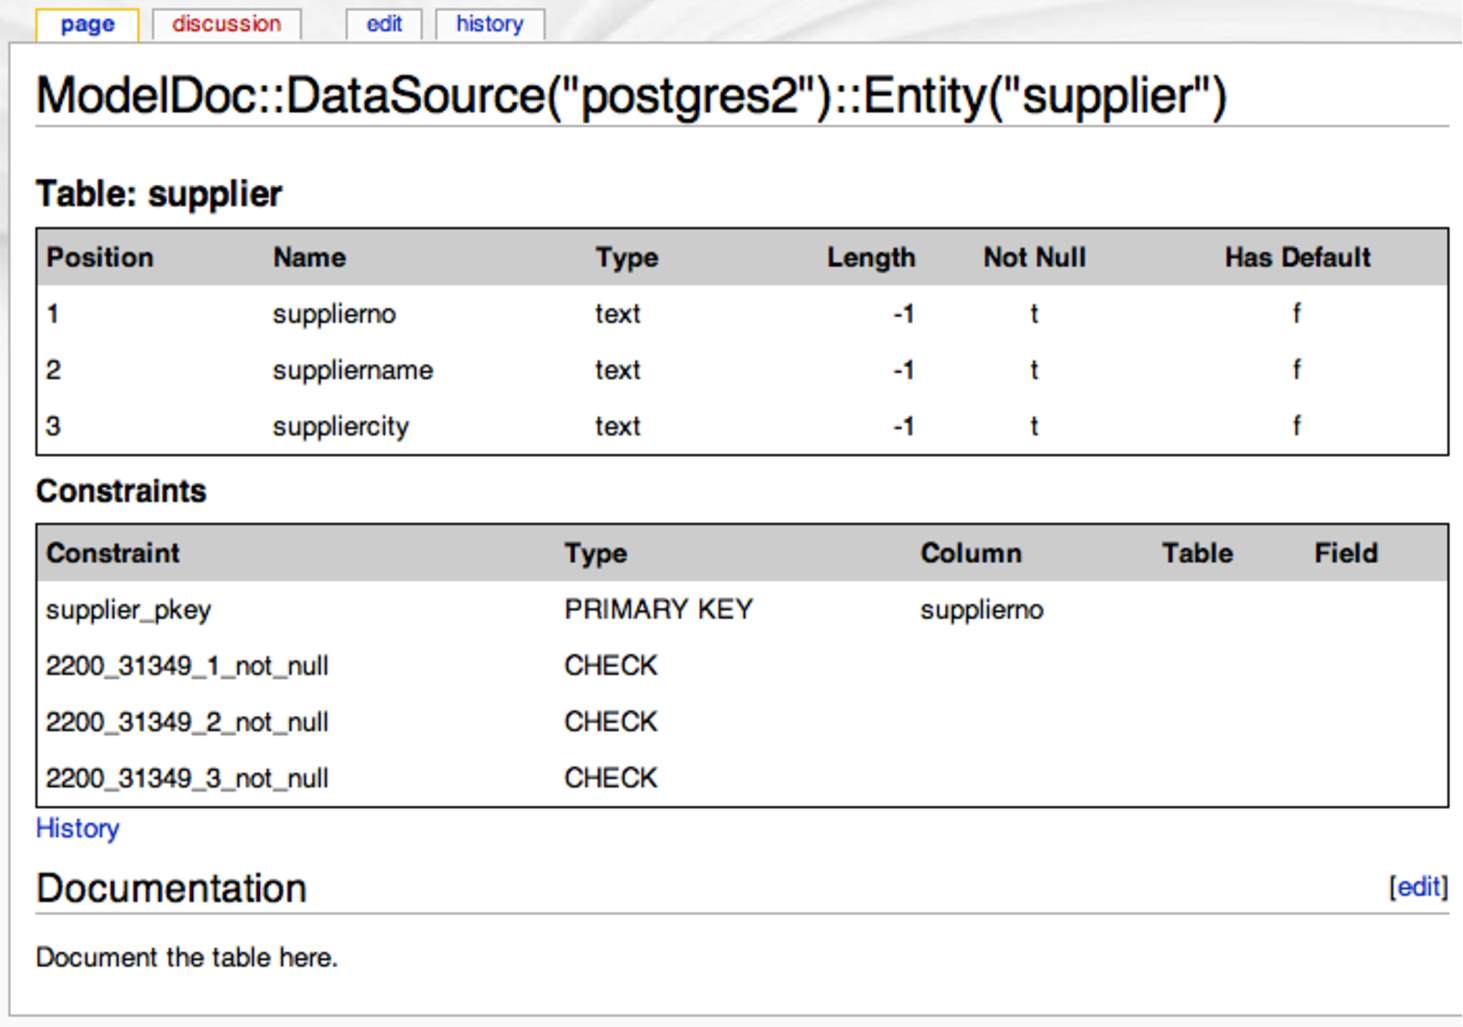
\includegraphics[width=220px]{entity-info.pdf}

\caption{A generated entity-info page.}

\end{figure}



\textbf{<entity-list datasourcename=``'' />}

Generates a table containing links to the entity-info page for each table in

the specified data source, as well as a link to the page documenting the data

source itself (which also contains this table).



\begin{figure}[ht]

\centering

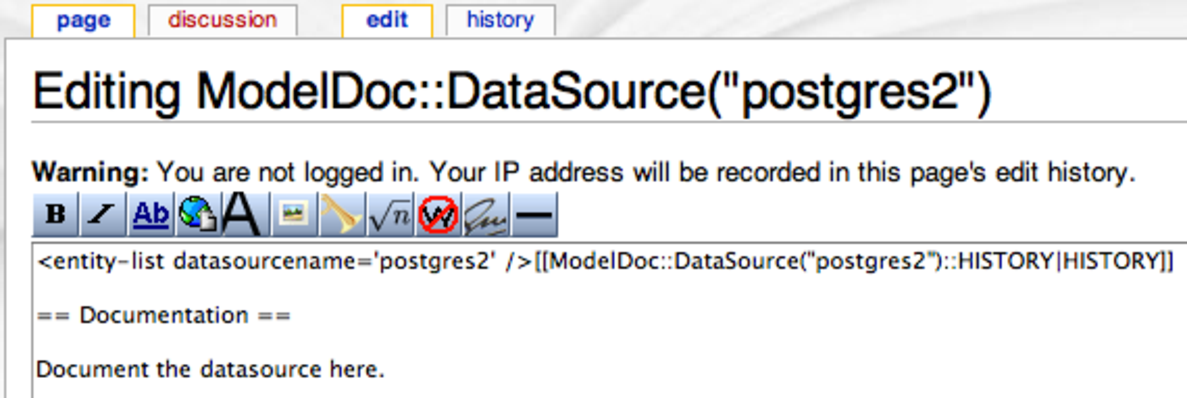
\includegraphics[width=220px]{entity-list-input.pdf}

\caption{A generated entity-list (data source) page.}

\end{figure}



\begin{figure}[ht]

\centering

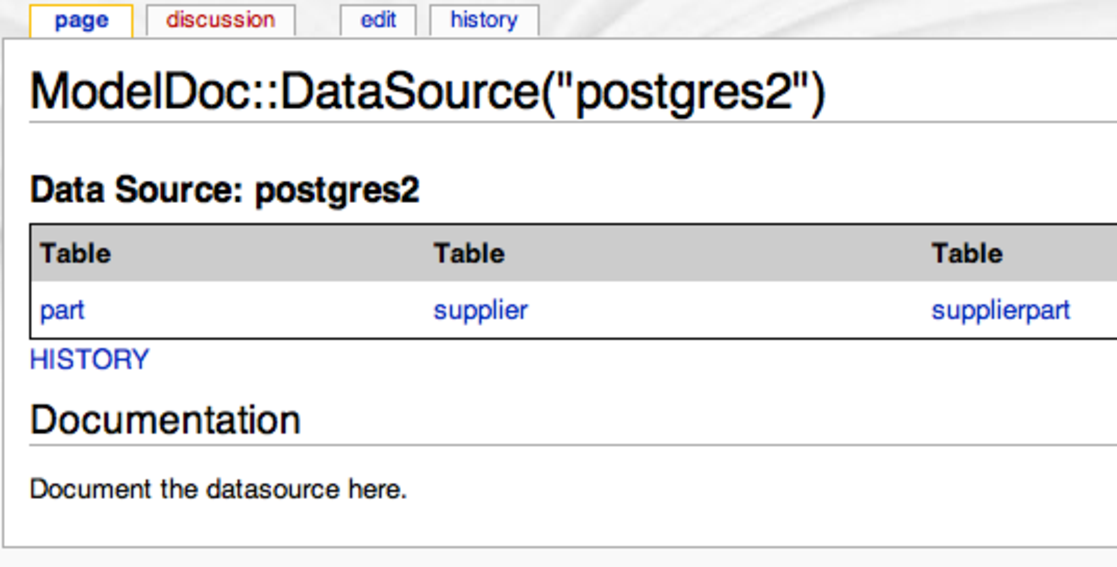
\includegraphics[width=220px]{entity-list-output.pdf}

\caption{The source of a generated entity-list (data source) page.}

\end{figure}



\textbf{<datasource-info datasourcename=``'' />}

Generates metadata on the specified data source



\textbf{<datasource-list />}

Generates a list of links to the datasource-info pages for all the registered

data sources.



\subsection{Special Pages}



\textbf{ModelDoc::Configuration}

This wiki-page contains XML specifying the data sources the wiki should be

connected to.



\begin{figure}[ht]

\centering

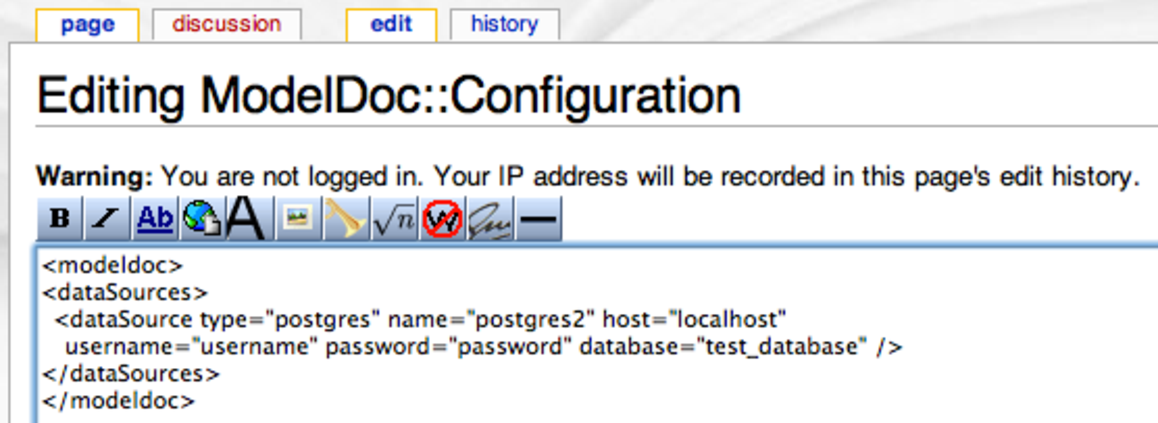
\includegraphics[width=220px]{configuration.pdf}

\caption{Example of the XML-based configuration page.}

\end{figure}



\textbf{ModelDoc::To Document}

This page maintains a ``todo"-list for

developers.  While we cannot automatically judge whether a change has been

properly been documented, we can track whether the page for a table has been

documented since the table was last updated.  We currently only track whether

the page has been updated at all, but this could be extended to further require

that a certain type of user (e.g. the database administrator), or a set of

users (e.g. the DBA as well as the UI designer and test writer) have

viewed/updated the content.  This serves to help avoid documentation becoming

stale because a developer changed code while forgetting to look at the

accompanying comments.



\textbf{ModelDoc::DataSource(``[name]'')}

This page provides links to all the entities found in that data source.  This

is also where users would provide documentation of the data source itself.



If changes to the data source are detected, an automated and editable

description of the change is appended to this page (and any designated users

are notified by e-mail).



A corresponding \textbf{ModelDoc::\ldots::HISTORY} page is

created along with this page that contains an XML description of the last-seen

metadata for the data source, including its list of tables.  This is the

baseline that ModelDoc compares the live database metadata to in order to 

detect changes.



\textbf{ModelDoc::DataSource\ldots::Entity\ldots}

This page displays the table's metadata, and provides a place for users to

document the table.



If changes to the table's metadata are detected (e.g. an added/removed column,

a changed constraint, etc.), an automated and editable description of the

change is appended to this page (and any designated users are notified

by e-mail).



As above, a corresponding

\textbf{ModelDoc::\ldots::HISTORY}

page stores the last-seen version of the table's metadata.



\section{Evaluation}



The performance overhead of using ModelDoc, examined in the next section, cannot

be ignored, though much of that overhead are a consequence of implementation

details that should be straightforward to overcome.  We also evaluate the

utility of ModelDoc by looking at defined database refactorings and how

ModelDoc would document them.



\subsection{Performance}



ModelDoc degrades the performance of a wiki in two primary ways: the disabling

of wiki-caching and the overhead of determining if a table has been updated

(and if so, updating the relevant pages). Both of these issues can be mitigated.



By default, MediaWiki uses an aggressive caching strategy.  Once a page has

been created/edited, the page is maintained in a cache for subsequent reads. 

This makes sense for the classical wiki-approach, wherein users edit static

content.  ModelDoc, however, currently requires that caching be disabled, so

that the content that a dynamic tag generates is not cached.  For example,

every time an entity-page is viewed, the corresponding table in the database is

examined and, if it has been updated, the page is updated to reflect this.  If

MediaWiki were allowed to cache this, the displayed data could fall out of

synch with the underlying database.



The algorithm for comparing table-metadata can add substantially to the

loading-time of a page.  The worst-case is the very first time a page is viewed

that contains an ``entity-list'' tag for a data source.  In this initial case,

the info/history pages for all the database tables are created.  Against a

ModelDoc installation on a MacbookPro (2.8 GHz Intel Core 2 Duo, 4 GB 1067 MHz

DDR3), using a database with 96 tables with an average of 7.3

columns and 2.8 constraints per table, this initial process took

an average of 4.08 minutes.  Fortunately, this only happens the first time, and

this should be done when ModelDoc is first installed by the administrator.



Thereafter, viewing an ``entity-list" page took an average of 33.36 seconds. The

difference is that wiki pages are not often being created/edited at that point

-- the bottleneck is primarily the database connections for retrieving the

current metadata, and retrieving the previously-cached metadata XML for the

table from its respective HISTORY wiki page.



Viewing an ``entity-info'' page -- and therefore refreshing the

version-information for only a single table, rather than for all of them --

took an average of 5.6 seconds.



We are in the process of moving this work into a background process that will

almost entirely mitigate these issues.  For many projects, a page being a

maximum of an hour, or even a day, outdated should be sufficient, especially if

the time-of-last-update is clearly displayed on the page.  Further, it would

then be a minor implementation detail to allow privileged users to kick off

the versioning-process manually at any time, so they could guarantee current

data when necessary.



\subsection{Usage}



We can use refactorings from \cite{ambler:refactoring} to both illustrate where

ModelDoc currently stands and where it can go with regard to where it can be

used in a database's evolution.



Any refactoring that reduces to the addition/drop of a table, column, or

constraint, are currently detected by ModelDoc.



The renaming of a table, for example, will be tracked by ModelDoc, but it will

be reflected as a table-deletion and a table-addition.  Similarly, ``moving'' a

column from one table to another will look like a column-removal and a

column-addition.



The tables in this section enumerate through the refactorings in

\cite{ambler:refactoring}, indicating whether a refactoring will be

indicated in a reasonably straightforward way (indicated with \checkmark, e.g.

``Drop Column''), the refactoring will be indirectly and/or poorly captured

(indicated with *, e.g. ``Merge Columns'', since this could ambiguously

appear as either a column deletion-and-addition, or simply a deletion), or the

refactoring will (essentially, at least) not be detected at all by ModelDoc.



As indicated, while ModelDoc documents structural changes well, it does not

capture refactorings that deal with the data itself, such as new

semantics or data-formats. Further, ModelDoc does not detect refactorings that

are made up of both column and table changes, such as the ``Replace Type Code

With Property Flags'' refactoring, which entails replacing a single

``code''-type column with multiple boolean columns, e.g. replacing an

``AddressType'' column with ``isHomeAddress'', ``isWorkAddress'', etc. columns.

ModelDoc also clearly needs to be extended to monitor stored procedures.



\begin{table}[h]

  \caption{Structural Refactorings}

  \centering

\begin{tabular}{ | l | c | }

  \hline

  \textbf{Refactoring} & \textbf{Detected} \\

  \hline

  Drop Column & \checkmark \\

  Drop Table & \checkmark \\

  Drop View & \checkmark \\

  Introduce Calculated Column & * \\

  Introduce Surrogate Key & * \\

  Merge Columns & * \\

  Merge Tables & * \\

  Move Column & \checkmark \\

  Rename Column & \checkmark \\

  Rename Table & \checkmark \\

  Rename View & \checkmark \\

  Replace LOB With Table & \\

  Replace Column & \checkmark \\

  Replace 1-to-Many With Assoc. Tbl & \checkmark \\

  Replace Surrogate Key With Natural Key & * \\

  Split Column & * \\

  Split Table & * \\

  \hline

\end{tabular}

\end{table}



\begin{table}[h]

  \caption{Data Quality Refactorings}

  \centering

\begin{tabular}{ | l | c | }

  \hline

  \textbf{Refactoring} & \textbf{Detected} \\

  \hline

    Add Lookup Table & * \\

    Apply Standard Codes & \\

    Apply Standard Type & \\

    Consolidate Key Strategy & \\

    Drop Column Constraint & \checkmark \\

    Drop Default Value & \checkmark \\

    Drop Non-Nullable Constraint & \checkmark \\

    Introduce Column Constraint & \checkmark \\

    Introduce Common Format & \\

    Introduce Default Value & \checkmark \\

    Make Column Non-Nullable & \checkmark \\

    Move Data & \\

    Replace Type Code With Property Flags & * \\

  \hline

\end{tabular}

\end{table}



\begin{table}[h]

  \caption{Referential Integrity Refactorings}

  \centering

\begin{tabular}{ | l | c | }

  \hline

  \textbf{Refactoring} & \textbf{Detected} \\

  \hline

    Add Foreign Key Constraint & \checkmark \\

    Add Trigger For Calculated Column & \checkmark \\

    Drop Foreign Key Constraint & \checkmark \\

    Introduce Cascading Delete & * \\

    Introduce Hard Delete & \\

    Introduce Soft Delete & * \\

    Introduce Trigger For History & * \\

  \hline

\end{tabular}

\end{table}



\begin{table}[h]

  \caption{Architectural Refactorings}

  \centering

\begin{tabular}{ | l | c | }

  \hline

  \textbf{Refactoring} & \textbf{Detected} \\

  \hline

    Add CRUD Methods & \\

    Add Mirror Table & \\

    Add Read Method & \\

    Encapsulate Table With View & * \\

    Introduce Calculation Method & \\

    Introduce Index & \checkmark \\

    Introduce Read-Only Table & \\

    Migrate Method From Database & \\

    Migrate Method To Database & \\

    Replace Method(s) With View & \\

    Replace View With Method(s) & \\

    Use Official Data Source & \\

  \hline

\end{tabular}

\end{table}



\begin{table}[h]

  \caption{Transformations}

  \centering

\begin{tabular}{ | l | c | }

  \hline

  \textbf{Refactoring} & \textbf{Detected} \\

  \hline

    Insert Data & \\

    Introduce New Column & \checkmark \\

    Introduce New Table & \checkmark \\

    Introduce View & \checkmark \\

    Update Data & \\

  \hline

\end{tabular}

\end{table}



\begin{figure}[h]

\centering

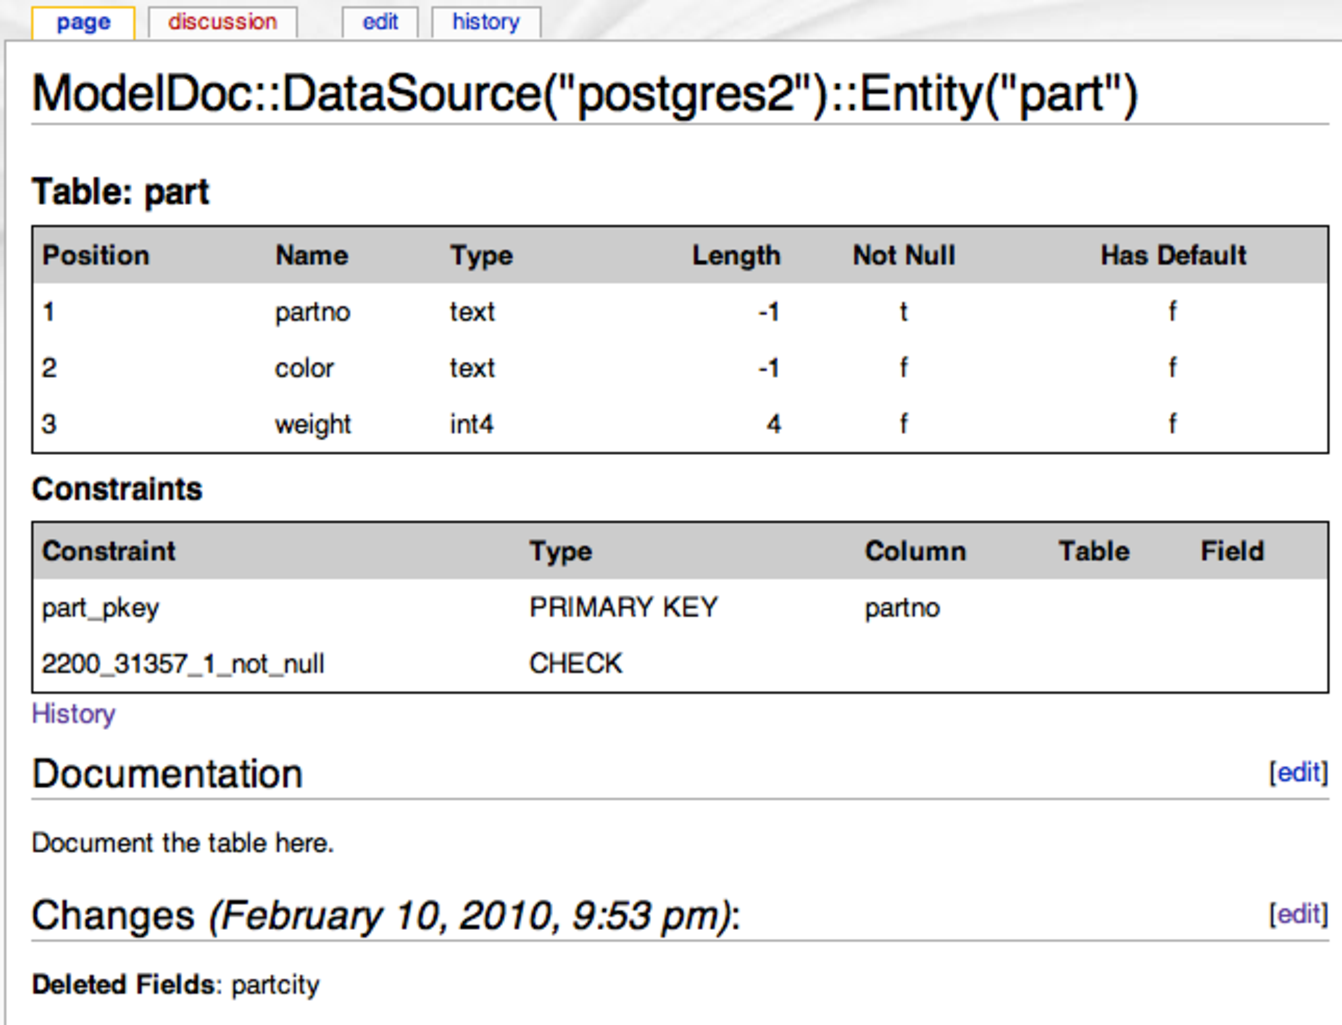
\includegraphics[width=220px]{drop-column.pdf}

\caption{The entity-info page after a dropped column is detected}

\end{figure}



\begin{figure}[h]

\centering

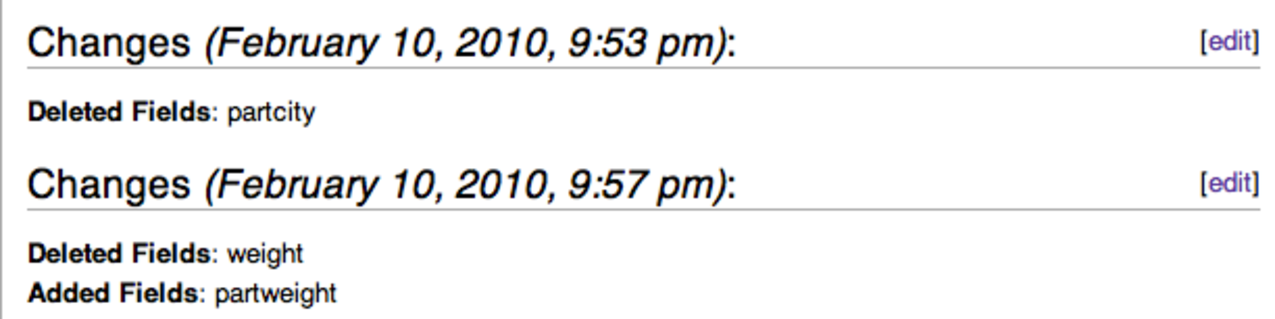
\includegraphics[width=220px]{rename.pdf}

\caption{The result of a column-rename}

\end{figure}



\section{Future Work}



\subsection{Database Visualization}



ModelDoc, being wiki-based, offers a web-flavored view of an application's

model.  To see how two entities are inter-related, users can examine the

hyperlinks between the two.  This can offer a very limited window, however,

when an application's entity-relationships make up a complex graph.



ModelDoc may be extended to incorporate better ways to understand and work with

the data.  For example, graph-visualization software, such as Graphviz

\cite{web:graphviz} or SchemaSpy \cite{web:schemaspy}, could be incorporated to

better-indicate where an entity fits in the larger scheme.



\subsection{Heterogeneous Databases}



While, at the time of this writing, a single ModelDoc installation can support

multiple databases, there is no automatic inter-linking between the

documentation generated between those databases.  An obvious challenge is that

since these data sources are created separately, the relationship between the

data in each cannot easily be inferred.  There has been

some work on auto-generating a user-friendly visualization of heterogeneous

database systems like this \cite{catarci:heterogeneous}.



\subsection{Inferring ModelDoc Semantics From User Documentation}



To achieve mutual-consistency between the human-documentation and the database

metadata, ModelDoc could be extended to infer, for example, that a user is

referring to a given entity even on a non-ModelDoc page.  If that entity

is updated, ModelDoc could then notify the user that this other

documentation may also need to be updated.



\subsection{Higher-Level Model Descriptions}



The model of an application is rarely exclusively contained in the database

schema.  Most applications contain an object model that abstracts on top of the

data model.  For example, as previously discussed, in a database a Person entity and its associated Address

may be normalized into two tables.  In the object-oriented application,

however, this relationship would take the form of a Person object composed with

an Address object.



While a DBA may be more interested in the database-view of the model, the

application developers (and perhaps the end-users as well) could stand to

benefit more from documentation at the object-abstraction level.



ModelDoc should be extended to document models at the source code

level, similar to Doxygen and JavaDoc solutions -- in fact, these other approaches

could likely simply be integrated.  By further incorporating version-control

and IDE support, this could become a very powerful tool for documenting source

code.



See the ``Architectural Refactorings'' table for further motivation for

extending support for taking the higher-level application layers into account:

some refactorings involve corresponding changes at multiple levels, and it

should be possible to clearly document these changes.



\subsection{Semantic Structure}



Currently, the data in the pages created by ModelDoc are semi-structured.  If

ModelDoc were extended to work with heterogeneous data sources, and also to

document multiple levels of abstraction, we would be providing a common

semi-structure to all these sources.  This could allow for semantic querying of

this data, similar to other semantic querying approaches such as that of

WolframAlpha \cite{web:wolfram}.



\subsection{Ability to Mutate Data Sources}



There is little current tool-support for performing database refactoring

\cite{ambler:refactoring}.  Instead of documenting in a read-only way, ModelDoc

could be used to allow mutation of the underlying data sources, including carrying out complex refactorings.  This would allow ModelDoc to know for sure that such

refactorings were intended -- a column-rename, for example, would no longer be

seen as a column-deletion and column-addition.s



\section{Discussion - Comparison to Source Code Documentation Generation}



Documentation generators such as Doxygen \cite{web:doxygen} and JavaDoc

\cite{web:javadoc} consume the static-structure of source code along with

annotated comments, and produce human-readable output in the form of HTML or

PDF.



Relational databases could be extended to allow more meta-documentation to be

stored along with the existing metadata.  Column names, for example, are often

not self-describing.  These comments could be used for tooling similar to above

generators.



On the other hand, source code documentation generators could be extended to

create/update a mini-wiki so that its documentation could be collaboratively

documented.



\section{Conclusions}

Motivated by the widespread lack of quality documentation, and the consequences

of that lack, we presented ModelDoc.  Combining the collaborative documentation

capabilities of MediaWiki with custom extensions, ModelDoc continuously

maintains a baseline level of documentation that is guaranteed to be in synch

with the database in use.



\bibliographystyle{abbrv}

\bibliography{modeldoc}

\balancecolumns



\end{document}
